
% Chapter 3 File

\chapter{Statistical Modeling and Methodology}
\label{chapter2}
\thispagestyle{empty}

\section{Latin Square Model and Specifications}
The Replicated Latin Square model (Case I) of size $p=4$ is a type of randomized complete block design that contains letters from the Latin alphabet in which each letter represents a treatment, which is the distance covered by hikers within a sixty-minute interval in the conducted experiment, each of the letters are randomly permuted and no single letter is repeated in the same row and column. This is synonymous with the design of Sudoku puzzles where each column and row entry is unique. The experiment considers three replications of the standard Latin Square design by fixing the nuisance factor levels and replicating the experiment over a given number of times. Three replications spread throughout a three consecutive day basis were considered. According to the Pennsylvania State University's Experimental Design and Analysis online textbook, this experiment is orthogonal due to the unique random permutation property of the Latin letters previously mentioned \cite{key2}. This allows the design to be easier and cleaner to analyze since interaction effects are not considered as relevant in the experiment. The model in terms of mathematical notation is given by:\\
\centerline{$y_{ijkl} = \mu + \tau_{i} + \rho_{j} + \beta_{k} + \delta_{l} + \epsilon_{ijkl}$}\\
\centerline{$i = 1,2,3,4 \\
j = 1,2,3,4 \\
k = 1,2,3,4\\
l = 1,2,3$}\\
Note that in this model, the iteration index j is dependent on i and k, which is denoted by j = d(i,k). This is the specific model for our experiment since the experiment will include four levels each of temperature and humidity respectively. The Greek letter $\mu$ denotes the overall mean distance within the sixty-minute time period. The next term in the above equation, denoted as $\tau_{i}$ is the ith "...". The following term is $\rho_{j}$ which is the jth level of the temperature block variable. $\beta_{k}$ is the kth level of the humidity percentage block variable. The term $\delta_{l}$ represents the lth replicate of the experiment in which the experiment was repeated for three consecutive days in which the same levels of both temperature and humidity were measured. Lastly, $\epsilon_{ijkl}$ is the random error term of the Latin Square model.\\\\
\section{Assumptions of the Latin Square Statistical Model}
In this section, the required assumptions and appropriate hypothesis tests are provided to better inform the reader of how the statistical analysis will be conducted. In this model, we assume that:\\
\centerline{$1. \sum_{i}^{4} \tau_{i} = 0$}
\centerline{$2. \sum_{j}^{4} \rho_{j} = 0$}
\centerline{$3. \sum_{k}^{4} \beta_{k} = 0$}
\centerline{$4. \sum_{l}^{3} \delta_{l} = 0$}
\centerline{$5. \epsilon_{ijkl} \overset{iid}{\sim} N(0,\sigma^2) $}\\\\
These assumptions indicate that the summation of each of the respective effects should be equal to $0$ and that the random error term of the Latin Squares model should be independently and identically distributed with a Normal distribution of mean $0$ and variance $\sigma^2$.\\\\
\section{Hypothesis Test of the Latin Squares Model}
For the analysis of the experiment, we consider the following set of hypotheses and the F test ratios\cite{key3}:\\
\centerline{$H_o: \tau_{i} = 0$}\newline
\centerline{$H_a: \tau_{i} \neq 0$}\newline
\centerline{$H_o: \rho_{j} = 0$}\newline
\centerline{$H_a: \rho_{j} \neq 0$}\newline
\centerline{$H_o: \beta_{k} = 0$}\newline
\centerline{$H_a: \beta_{k} \neq 0$}\newline
\centerline{$H_o: \delta_{l} = 0$}\newline
\centerline{$H_a: \delta_{l} \neq 0$}\newline
\centerline{$F^* = \frac{MS_{trt}}{MS_{E}}$}\newline
\centerline{$F^* = \frac{MS_{row}}{MS_{E}}$}\newline
\centerline{$F^* = \frac{MS_{col}}{MS_{E}}$}\newline
\centerline{$F^* = \frac{MS_{rep}}{MS_{E}}$}\\
The F test ratio value $F^*$ is the mean squared value for the treatments divided by the mean squared value for the error within the model. The other F test ratios are calculated similarly with the respective mean square values of each model component. The calculations of the mean square values will be elaborated on in the following section. The null hypothesis produces the inference that the mean treatment effects are insignificant, while the alternative hypothesis produces the inference that the mean treatment effects differ. For this experiment, the significance level is set to the default $\alpha = 0.05$ when the hypothesis test is conducted using the data from the analysis of variance (ANOVA) table.\\
We reject the null hypothesis $H_o$ if the F test ratio value is greater than the F critical value. This leads to the conclusion that the mean distance effects are statistically significant, meanwhile, if the F test ratio value is less than the F critical value, the appropriate conclusion is that we fail to reject the null hypothesis $H_o$ and conclude that the mean distance effects are statistically insignificant. The full ANOVA table that was outputted from the computer is provided in the appendix section.

\section{Estimation of Effects and Generalization of the Replicated Latin Squares ANOVA Table}
The effects from the generalized linear model can be estimated using the following formulas:\\
\centerline{$\hat{\mu} = \overline{y}....$}\newline
\centerline{$\hat{\tau_{i}} = \overline{y}_{i...} - \overline{y}_{....}$}\newline
\centerline{$\hat{\rho_{j}} = \overline{y}_{.j..} - \overline{y}_{....}$}\newline
\centerline{$\hat{\beta_{k}} = \overline{y}_{..k.} - \overline{y}_{....}$}\newline
\centerline{$\hat{\delta_{l}} = \overline{y}_{...l} - \overline{y}_{....}$}\\
The estimate for the overall mean distance effect is the grand mean of the data set which is calculated by adding all the observations in the data and dividing by the total number of observations. The treatment effect estimate is calculated by subtracting the mean of the ith treatment group by the grand mean. Similarly, the temperature block effect is calculated by calculating the difference between the jth row average and the grand mean. For the humidity level block effect, the difference between the kth column average and the grand mean is calculated. Finally, the estimate for the replicate day effect is found by subtracting the lth replicate mean by the grand mean. Note that these averages are taken of the data collected in the experiment being analyzed. We provide these estimates in the respective appendix section. Provided below is a brief summary of the replicated Latin Square (Case I) design ANOVA table. In this table, $p$ represents the size of the Latin Square, $n$ correlates to the number of replications, and the total sum of squares of the data is denoted by $SS_{T}$. For notation convenience and ease, these are the conventional symbols that will be used when analyzing the calculations from the computer output in the following chapter.\\
\begin{figure}[htp]
    \centering
    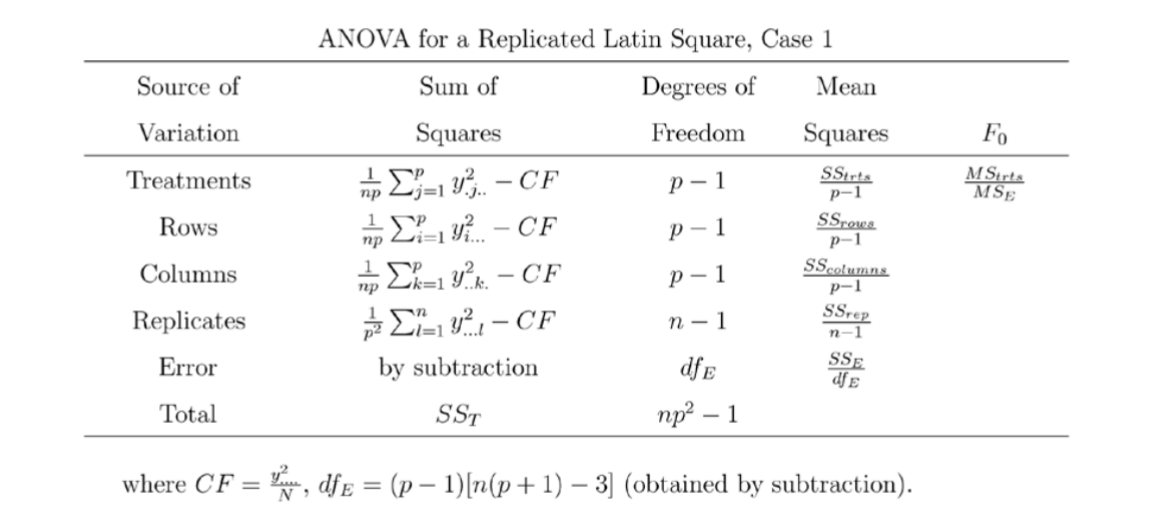
\includegraphics[width=150mm]{ANOVA_RepLS.png}
    \caption{The generalized Analysis of Variance table for the Replicated Latin Square Design (Case I)}
    \label{fig:ANOVA_Repls}
\end{figure}